\section{ Gilbert-Peierls' Algorithm}

Gilbert-Peierls' algorithm \cite{GPAlgo} (\ref{algo:GP}) provides a method to achieve LU decomposition with partial 
pivoting in time proportional to \bigo{flops(LU)}, i.e. number of floating point
operations \cite{GPAlgo}. It is a left looking algorithm because it computes the \(k^{th}\)
column of L and U using the previously computed \((k-1)\)  columns of L matrix. The notations used in the 
algorithm are as follows: $j$ is the index of the column of $L$ and $U$ being compute.
Unprimed variables mean the section of the matrix or vector above the row with index $j$.
Primed variables represent the section of matrix or vector below the row index $j$ including 
the $j^{th}$ row. thus vector $a_j = (a_{1,j}, a_{2,j}, \dots, a_{j-1,j})^T$ and 
vector $a'_j = (a_{j,j}, \dots, a_{n,j})^T$,
$$ L_j = 
\begin{bmatrix}
    l_{1,1} & \dots & o \\
    \vdots & \ddots  & \vdots \\
    l_{j,1} & \dots & l_{j-1, j-1}
\end{bmatrix} \ L'_l = 
\begin{bmatrix}
    l_{1,j} & \dots & l_{j, j-1} \\
    \vdots & \ddots  & \vdots \\
    l_{n,1} & \dots & l_{n, j-1}
\end{bmatrix}
$$
The naming conventions in general are explained the figure \ref{fig:GP:namingConvention}. \\

\begin{algorithm}
    \caption{Gilbert-Peierls Algorithm: A Column-Oriented LU Factorization
        \label{algo:GP}}
    \begin{algorithmic}[1]
        \Require{$A$, a $n\times n$ asymmetric matrix}
        \Statex
        \State $L := I$
        \For{$j := 1 \textrm{ to } n$}
            \Comment{Compute $j^{th}$ column of $L$ and $U$}
            \State Solve $L_j u_j = a_j$ for $u_j$
            \State $b'_j := a'_j - L'j u_j$
            \State Do Partial Pivoting on $b'j$
            \State $u_{jj} := b_{jj}$
            \State $l'_j := b'_j / u_{jj}$
        \EndFor
    \end{algorithmic}
\end{algorithm}


The central idea of the Gilbert-Peierls' algorithm \cite{GPAlgo} is to solve the lower triangular
system \(Lx = b\) where \(L\) is a lower triangular matrix and \(x,\ b \) are 
spare column vectors (Algorithm \ref{algo:GP_tri}). This method requires to pre-compute the location of all
the non-zero elements in the sparse column vector $x$, which is referred as 
\textit{Symbolic Analysis}. This step has to repeated for all the $n$ column of 
the matrix $A$.


\begin{figure}
    \centering
    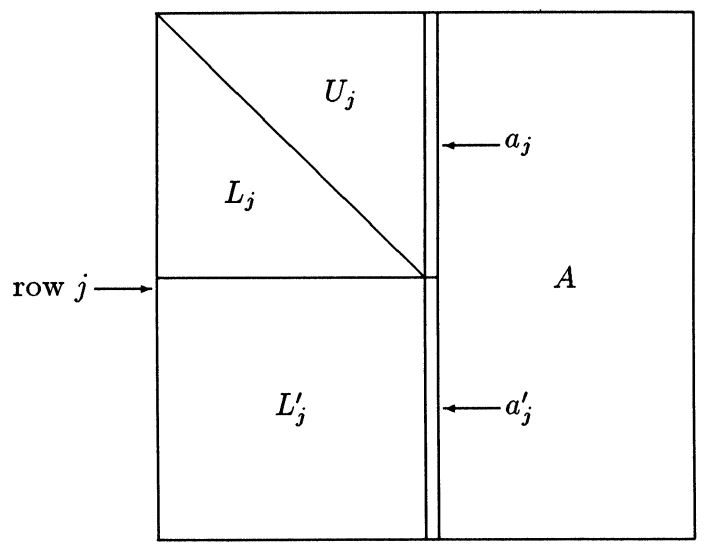
\includegraphics[width = 0.55\textwidth]{./Theory/gpConvention.JPG}
    \caption{Naming conventions used in algorithm \ref{algo:GP}}
    \label{fig:GP:namingConvention}
\end{figure}

\pagebreak

\section{Symbolic Analysis}
% \label{sec:GP:symbolic}

Symbolic analysis is a process to determine the set of non-zero locations ($\chi$)
in solving the lower triangular system $L_j x = b$, where $J_j$ is a unit diagonal 
lower triangular matrix representing only first ($j-1$) columns. Listing all 
the non-zero locations \(\chi\) gives the numerical computation time proportional to
the number floating point operations i.e. \bigo{f},

\begin{algorithm}
    \caption{Gilbert-Peierls Algorithm: Solving a Dense Triangular System $L_j x = b$
        \label{algo:GP_dense_tri}}
    \begin{algorithmic}[1]
        \Require{$L_j$ is a dense lower triangular matrix, $x, b$ are sparse column vectors}
        \Statex
        \State $x := b$
        \For{$k = 1$ to $j-1$}
            \State $x := x - x_{i}  (l_{1,i}, l_{2,i}, \dots, l_{j-1,i})$
        \EndFor
    \end{algorithmic}
\end{algorithm}

The algorithm \ref{algo:GP_dense_tri} represents the process of solving a dense 
lower triangular system. In sparse systems some of the $b$ entries and $L_j$ entries
are zero resulting in no change and hence can be eliminated. Algorithm \ref{algo:GP_tri} 
represents the sparse version of the algorithm 

\begin{algorithm}
    \caption{Gilbert-Peierls Algorithm: Solving Triangular System $L_j x = b$
        \label{algo:GP_tri}}
    \begin{algorithmic}[1]
        \Require{$L_j$ is a lower triangular matrix, $x, b$ are sparse column vectors}
        \Statex
        \State $x := b$
        \For{$\textrm{ each } j \in \chi$}
            \For{$\textrm{ each } i > j \textrm{ for which } l_{ij} \neq 0$}
                \State $x_i := x_i - l_{ij} x_j$
            \EndFor
        \EndFor
    \end{algorithmic}
\end{algorithm}

\begin{figure}[H]
    \centering
    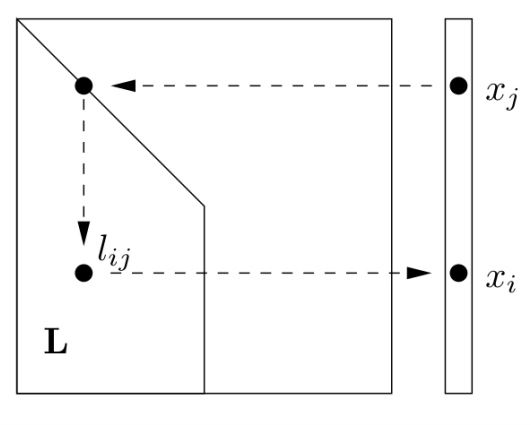
\includegraphics[width = 0.55\textwidth]{./Theory/nnzPattern.JPG}
    \caption{Non-zero pattern in LU decomposition}
    \label{fig:GP:nnzPattern}
\end{figure}

\pagebreak

Lines 1 and 3 of the algorithm \ref{algo:GP_dense_tri} suggests that the element
of the result vector ($x_{ij}$) can become non-zero only of the corresponding element in the
vector $b$ ($b_{i}$) is non-zero or there exits a non-zero element $l_{i,j}$ where 
$j$ is less than $i$ and $x_{j}$ is non zero. 

\begin{subequations}
    \centering
    \begin{align}
        (b_i \neq 0) &\implies (x_i \neq 0) \\
        (x_j \neq 0) and \exists i(l_{ij} \neq 0) &\implies (x_i \neq 0)
    \end{align}
    \label{eqn:GP:findingX}
\end{subequations}

These two implications can can be visualized using the figure \ref{fig:GP:nnzPattern}.
In the column factorization algorithms like Gilbert-Peierls, we know the locations of all the 
non-zero elements for the columns with indices lower than $j$ we can determine 
the non-zero locations ($\chi$) before solving for that column and for the entire
lower triangular system.



